% !TEX root = task4.tex
% -----------------------------------------------------------------
% Filename  :	task4_stateMachine_writeAllocatePolicy.tex
% Author    :	Carsten Hoppe
% Date		:	28. Januar 2017
% Reference	:	http://www.texample.net/tikz/examples/state-machine/
%				https://martin-thoma.com/how-to-draw-a-finite-state-machine/
% -----------------------------------------------------------------
%\tikzstyle{every state}=[fill=mycolor,text=white,minimum width=2cm]
After we have implemented the direct mapped cache, we have to design a finite state machine for the cache controller. This controller have to count the cache hits and cache misses using counters, which are reset at program start. On the one hand, we implement the write back policy. On the other hand, we implement the write allocate policy.\\
In figure \ref{tik:FSM} the state diagram of the cache controller is illustrated. The state diagram represents a Mealy automaton. Besides the state machine inputs are listed in table \ref{tab:tableFSMInputs} and the state machine outputs are shown in table \ref{tab:tableFSMOutputs}. A sketch of the state diagram is printed in figure \ref{fig:sketchMealyAutomata}.\\
In the following, we describe the state space of the state machine:
\begin{itemize}
	\item[IDLE] This state is the initial state of the state machine. When the cache is reset and state machine switches to this state.
	\item[CHECK1] In this state, the cache is checking whether write operation will results in a cache hit or not. Thus, the valid bit, dirty bit and the tag values of the correspondent cache block line are relevant for checking cache hit or cache miss.
	\item[CHECK2] In this state, the cache is checking whether read operation will results in a cache hit or not. Thus, the valid bit, dirty bit and the tag values of the correspondent cache block line are relevant for checking cache hit or cache miss.
	\item[WRITEBACK1] When checking the current cache block line results in a cache miss, and the current cache block line is dirty, this cache block line must be written back to the main memory first. Inside this state, the cache writes the cache block line back to the main memory. The process of writting back requires a specific number of clock cycles. Thus, we have to wait for the main memory. If the main memory signalizes that it is ready, then we can change this state to the next state.
	\item[WRITEBACK2] When checking the current cache block line results in a cache miss, and the current cache block line is dirty, this cache block line must be written back to the main memory first. Inside this state, the cache writes the cache block line back to the main memory. This process of writting back requires a specific number of clock cycles. Thus, we have to wait for the main memory. If the main memory signalizes that it is ready, then we can change this state to the next state.
	\item[WRITE] Before we will write the new data word into the cache, we have to read the cache block line from the main memory into the cache. While the cache is reading from the main memory, we stay in this state. When the main memory is ready and the cache finished reading from the main memory, we switch the current state.
	\item[READ] In case of a cache miss, we have to read the correspondent cache block line from the main memory into the cache. While the we are reading from the main memory, we are inside this state. The main memory signalizes via a correspondent signal if the read operation is finished.
	\item[TOCACHE1] When the write operation has been finished, we achieve this state of the state machine. This state is necessary to increment the miss counter by one. 
	\item[TOCACHE2] When the read operation has been finished, we achieve this state. This state is necessary to increment the miss counter by one. Also, we transmit the requested data word from the cache to the CPU.
\end{itemize}


\newpage
\begin{landscape}
\begin{figure}
	\centering
	\caption{State diagram of the cache controller.}
    \label{tik:FSM}
	\fcolorbox{blue}{myOrange}{
	\begin{tikzpicture}[->,>=stealth',shorten >=1pt,auto,semithick,/tikz/initial text=Reset]
                    
	% ------------------------------------------------------------------------------
    % Definition of tikz styles.       
	% ------------------------------------------------------------------------------
	\tikzstyle{vertex}=[state,fill=mycolor,text=white,minimum width=1cm]
	\tikzstyle{edge}  =[draw,thick,->, midway, above, sloped, font=\tiny]
	\tikzset{invisible/.style={minimum width=0mm,inner sep=0mm,outer sep=0mm}}
	
	% ------------------------------------------------------------------------------
	% Definition of nodes.
	% ------------------------------------------------------------------------------
	[align=center,xscale=1,node distance=2cm and 4cm]
	\node[initial,vertex]	(A)                    		{\tiny $IDLE$};
  	\node[vertex]         	(B) [below  left=5cm of A] 	{\tiny $CHECK1$};
  	\node[vertex]			(C) [below right=5cm of A]	{\tiny $CHECK2$};
  	\node[vertex]         	(D) [below  left=4cm of B] 	{\tiny $WRITEBACK1$};
  	\node[vertex]         	(E) [below right=4cm of C] 	{\tiny $WRITEBACK2$};
  	\node[vertex]         	(F) [below right=4cm of D] 	{\tiny $WRITE$};
  	\node[vertex]			(G) [below  left=4cm of E]  {\tiny $READ$};
  	\node[vertex]		    (H) [below  =2cm of F]  {\tiny $TOCACHE1$};
  	\node[vertex]			(I) [below =2cm of G]  {\tiny $TOCACHE2$};
  	\node	(J) [below =9cm of A,invisible]	{};

	% ------------------------------------------------------------------------------
	% Definition of paths.
	% ------------------------------------------------------------------------------
	\path (A) [edge] 	edge [bend right] node 	{wrCPURequest/-} 	(B)
	      (A) [edge]	edge [bend  left] node  {rdCPURequest/-}	(C)
	      (B) [edge]	edge [bend right] node  {hit / rHitCt++, data2Cache} (A)
	      (C) [edge]	edge [bend left ] node  {hit / rHitCt++, data2CPU} (A)
	      (B) [edge]    edge [bend left ] node  {lineIsNotDirty / rdMEM='1'} (F)
	      (B) [edge]    edge [bend right] node  {lineIsInvalid / rdMEM='1'} (F)
	      (B) [edge]	edge			  node	{lineIsDirty / cacheLine2MEM} (D)
	      (D) [edge]	edge 			  node	{readyMEM / rdMEM='1'} (F)
	      (F) [edge]	edge			  node	{readyMEM / wrNewCBLine} (H)
	      (H) [edge] 	edge [bend right] node 	{- / rMissCt++, data2Cache} (J)
	      (C) [edge]	edge 			  node  {lineIsDirty / cacheLine2MEM} (E)
	      (C) [edge]	edge [bend right] node  {lineIsInvalid / rdMEM='1'} (G)
	      (C) [edge]	edge [bend left ] node  {lineIsNotDirty / rdMEM='1'} (G)
	      (E) [edge]	edge 			  node	{readyMEM / -} (G)
	      (I) [edge]	edge [bend left ] node	{- / rMissCt++, data2CPU} (J)
	      (G) [edge]	edge 			  node  {readyMEM / -} (I)
	      (J) [edge]	edge 			  node  {} (A)
	      (E) [edge,loop right] edge	  node  {!readyMEM / -} (E)
	      (G) [edge,loop left]  edge	  node  {!readyMEM / -} (G)
	      (D) [edge,loop left] edge 	  node	{!readyMEM / -} (D)
	      (F) [edge,loop right] edge	  node  {!readyMEM / -} (F);
	      		
\end{tikzpicture}}
\end{figure}
\end{landscape}
\newpage

\begin{table}
	\caption{Overview - FSM Inputs}
	\label{tab:tableFSMInputs}
	\begin{tabular}{lll}
	\hline % \topline
	Abbreviation & Name & Description \\
	\hline % \midrule
	rdCPU 		& CPU Read Request			& - \\
	wrCPU 		& CPU Write Request 		& - \\
	cacheMiss 	& Cache Miss 				& - \\
	cacheHit	& Cache Hit					& - \\
	readyMEM 	& Write-Back is resolved 	& - \\
	isDirty		& Cache Block is dirty		& - \\
	\hline % \bottomrule
	\end{tabular}
\end{table}
	
\begin{table}
	\caption{Overview - FSM Outputs}
	\label{tab:tableFSMOutputs}
	\begin{tabular}{lll}
	\hline % \topline
	Abbreviation & Name & Description \\
	\hline % \midrule
	stallCPU		& Stall Processor				& - \\
	setDirty		& Set Dirty Bit (Modified) Bit 	& - \\
	wrMEM			& Write To Memory				& Write Replaced Block To Memory \\
	dataCPU			& Read Data Into CPU			& - \\
	rdMEM			& Read Cache Block Into Cache From Memory & - \\
	dataCPU2Cache	& Write Data Into Cache			& - \\
	\hline % \bottolrule
	\end{tabular}
\end{table}

\newpage
\begin{landscape}
\begin{figure}
	\centering
	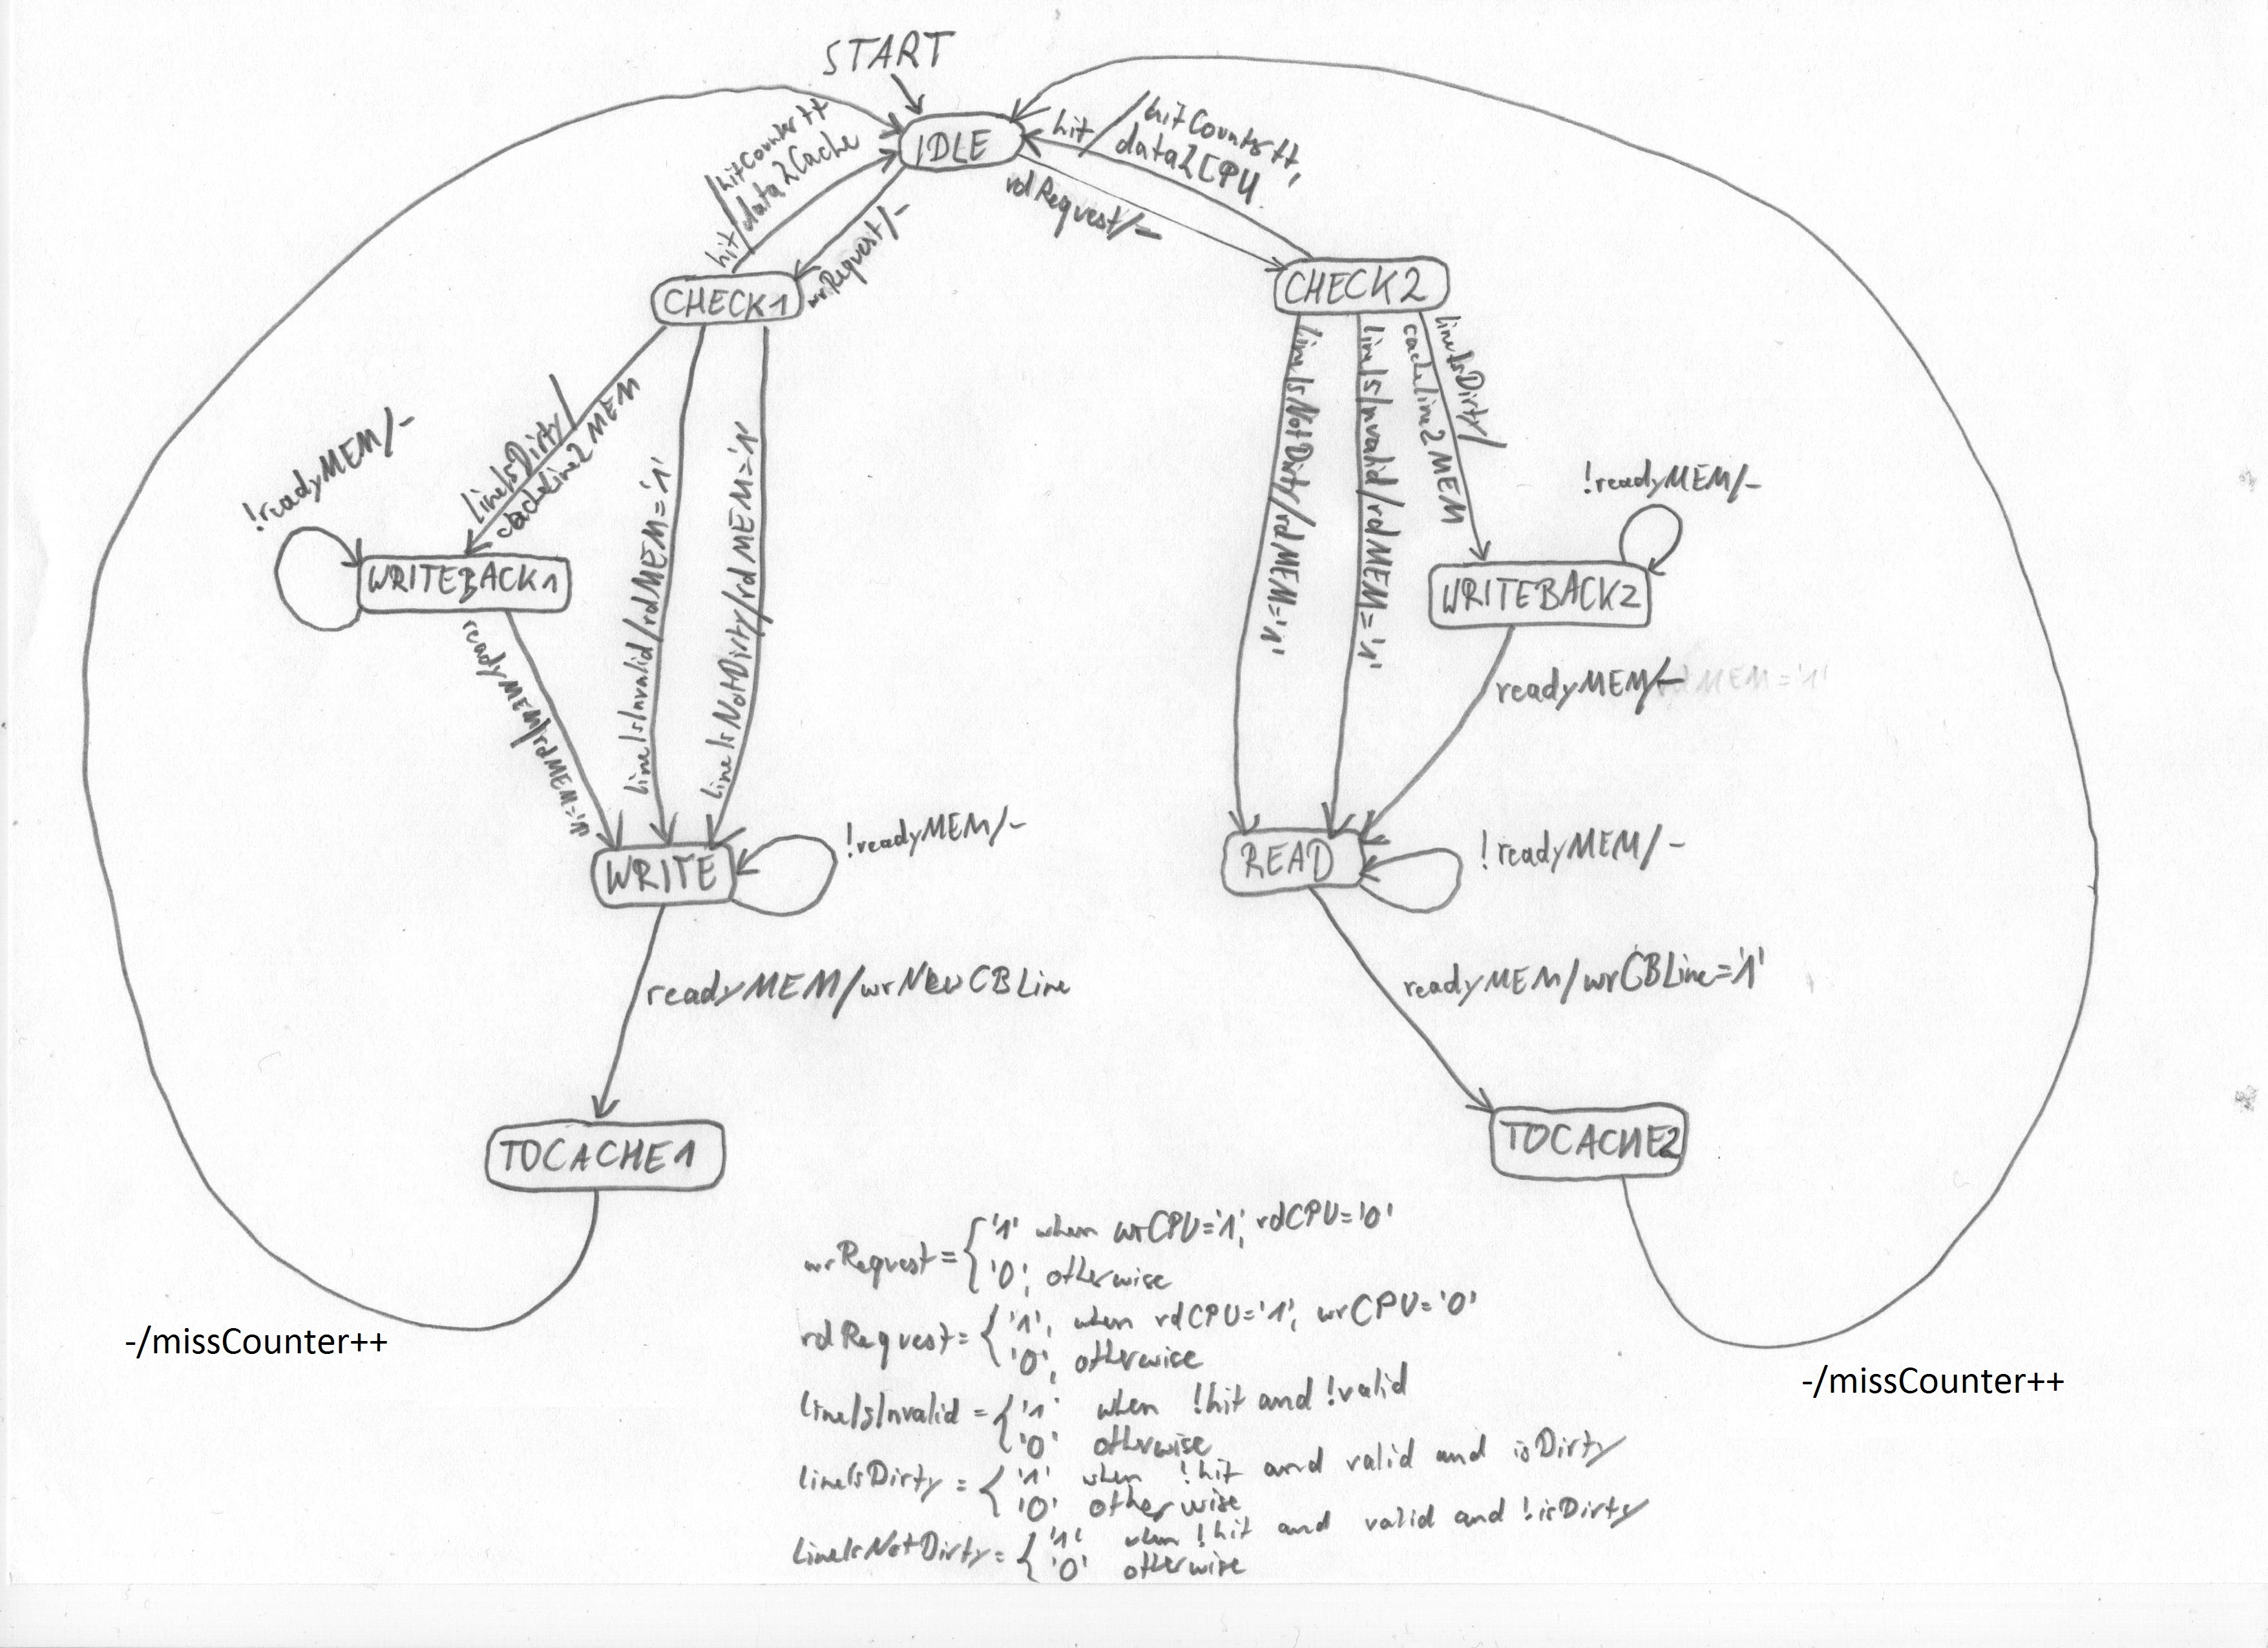
\includegraphics[scale=.8]{pictures/sketch_mealyAutomata_v2_modified}
	\caption{Sketch of Mealy Automata - Cache Controller, Version 2}
	\label{fig:sketchMealyAutomata}
\end{figure}
\end{landscape}